\documentclass[11pt,a4paper,oneside]{article}
\usepackage[dutch]{babel}
\usepackage{amsmath}
\usepackage{graphicx}
\usepackage{tikz}
\usepackage{fancyhdr}
\usepackage{dsfont}
\usepackage{parskip}
\usepackage{epstopdf}
\usepackage{listings}
\usepackage{color}
\definecolor{lichtgrijs}{gray}{0.95}
\usepackage{cite}
\usepackage[nottoc]{tocbibind}
\usepackage[T1]{fontenc}
\usepackage[light,math]{iwona}
\usepackage{pgfplots}
%\pgfplotsset{compat=newest}
\usepackage{subfig}
\usepackage{textcomp}
\usetikzlibrary{arrows,automata}
\usepackage{float}
\usepackage{longtable}
\usepackage{titling,enumitem}
\usepackage{a4wide}
\usepackage{amssymb}
\usepackage{rotating}
\usepackage{listings}
\usepackage[top=1.1in, bottom=1.2in, left=1.1in, right=1.1in]{geometry}
\usepackage{array}
\usepackage{titling}
\usepackage{blindtext}
\usepackage{chngpage}
\usepackage{calc}
\definecolor{lightgray}{gray}{0.8}
\newcolumntype{L}{>{\raggedleft}p{0.50\textwidth}}
\newcolumntype{R}{p{0.8\textwidth}}
\newcommand\VRule{\color{lightgray}\vrule width 0.5pt}
\usepackage{color, colortbl}
\definecolor{Gray}{gray}{0.9}
\definecolor{dkgreen}{rgb}{0,0.6,0}
\definecolor{gray}{rgb}{0.5,0.5,0.5}
\definecolor{mauve}{rgb}{0.58,0,0.82}
\definecolor{ugentblue}{rgb}{0.05,0.18,0.37}
\usepackage{import}
\usepackage[T1]{fontenc}
\begin{document}

%\newgeometry{top=0.8cm, right=1.70cm, left=1.7cm}
\begin{titlepage}

\thispagestyle{fancy}
\fancyhf{}
\fancyfoot[L]{}
\begin{figure}[!ht]
  \begin{adjustwidth}{-\oddsidemargin-1in}{-\rightmargin}
    \centering
    
\includegraphics[width=\paperwidth]{banner}
  \end{adjustwidth}
\end{figure}
\vspace{-0.2em}
\begin{center}
\vspace{5cm}
\Huge \textbf{Vakoverschrijdend Project: team Edran\\ Rapport episode 4}\\
\vspace{6.0cm}
\large
\begin{tabular}{L! {} R}
& {\LARGE\bf Team Edran} \\
& \\
& {\bf Steven De Blieck} \\
& {\bf Laurens De Graeve} \\
& {\bf Bart Middag} \\
& {\bf Wouter Pinnoo} \\
& {\bf Robin Praet} \\
& {\bf Stijn Seghers} \\
& {\bf Wouter Termont} \\
& {\bf Gilles Vandewiele} \\
\end{tabular}
\end{center}
\end{titlepage}
%\restoregeometry
\newpage

\fancyheadoffset[RO,LE]{0in}
\fancypagestyle{plain}{
\fancyhead[L]{Rapport episode 4}
\fancyhead[R]{Team Edran}
\fancyfoot[L]{}
\fancyfoot[R]{\thepage}}

\fancyhead[L]{Rapport episode 4}
\fancyhead[R]{Team Edran}
\fancyfoot[L]{}
\fancyfoot[C]{\thepage}
\pagestyle{fancy}
\tableofcontents
\newpage

\setcounter{section}{0}
\setcounter{subsection}{0}
\part{Verwachte functionaliteiten}
In deze episode is het enerzijds belangrijk de resterende nodige functionaliteiten te implementeren. Daarnaast is het ook belangrijk om de bestaande functionaliteiten te gaan optimaliseren, testen, bijsturen en documenteren.
\begin{itemize}
	\item Het moet mogelijk zijn voor een autobeheerder om een nieuwe auto toe te voegen tijdens of na de registratie
	\item Defini\"eren van een zone bij registratie, zoeken op zone bij lenen van auto's.
	\item Dashboard voor elke soort gebruiker. Dit is het eerste wat de gebruiker ziet en is key voor de UX!
	\item Mogelijkheid schadedossiers te doorzoeken op gebruiker en auto.
	\item Elke gebruiker heeft een userpage met daarin telefoonnummer, adres, auto's, reservaties, etc.
		\item   Re-designed admin-pagina. Betere onderverdeling in tabbladen voor de UX en overbodige tabbladen schrappen.
	\item Facturisatie afwerken gebaseerd op de criteria die we kregen van de klant.
	\item Mogelijkheid om niet alleen pdf te genereren maar ook een Excel-file.
	\item Een piechart module gebruiken om de statistieken beter visueel weer te geven.
	\item Layout uniform maken over heel de app.
	\item Zorgen dat geen onmogelijke data kan geselecteerd worden bij reservaties.
	\item E-mails zenden bij belangrijke ongelezen notificaties.
	\item Uniforme package names.
	\item DAO's meer generisch maken om bugs te voorkomen.
	\item Huidige e-mails effectief als een 'template' gebruiken. Bepaalde templates mogen niet verwijderd worden (bv. template voor registratie, wachtwoord vergeten, etc.)
	\item Tests schrijven voor de notificatie-module.
	\item De app populeren met mooiere data.
	\item Alle JS herschrijven naar JQuery zodat er cross-browser compatibiliteit is.
	\item Diverse bugs oplossen en opnieuw testen. 
	
\end{itemize}

\setcounter{section}{0}
\setcounter{subsection}{0}
\part{Usecases}
\section{Beschrijving}
\subsection{Nieuwe auto toevoegen tijdens of na het registreren}
Een nieuwe auto-eigenaar voert bij de registratie z'n basisgegevens in. Hij kan daarna optioneel nog zijn autogegevens toevoegen. Indien hij dat liever later doet, kan dat via een knopje in het menu dat enkel voor nieuwe auto-eigenaars zichtbaar is.

\subsection{Zone kiezen bij auto lenen}
Bij het lenen van een auto kan gefilterd worden op eerst en vooral de datum. Vervolgens op naam van de auto, aantal zitplaatsen, trekhaak, gps en nu ook de zone. De zones representeren een opdeling van de regio in een aantal gebieden.

\subsection{Dashboard om vlot te navigeren naar de belangrijkste functionaliteiten voor iedere soort gebruiker}
Het dashboard is de centrale plaats voor elke soort gebruiker (admin, nieuwe autolener, autolener, nieuwe autoeigenaar en autoeigenaar). Het doel van het dashboard is de gebruiker enerzijds herinneren aan de voornaamste acties die hij moet ondernemen (vaak tegen een bepaalde tijd) en anderzijds de meest gebruikte functies met zo weinig mogelijk kliks beschikbaar stellen. Daarnaast kan iedere gebruiker ook z'n statistieken bekijken hier.

\subsection{Duidelijkere keuzes voor de admin}
De admin heeft nu de keuze tussen volgende opties voor het beheer: Gebruikers, E-mail-voorkeuren, Notificatie voorkeuren, Schade en Afrekeningen. Dit betekent dat 'Bewijsmateriaal' en 'Schadedossiers' nu zijn samengevoegd onder 'Schade'. Het tabblad 'Facturisatie' is verwijderd want dit gebeurt automatisch door het systeem. De 'Verstuur Bericht' optie kan vanaf nu bij het bekijken van een gebruiker zijn profiel, wat deze episode ook toegevoegd wordt.

\subsection{Schadedossiers doorzoeken per gebruiker en per auto}
Het moet voor een admin mogelijk zijn om schadedossiers rap terug te vinden. De criteria die hij hierbij kan kiezen zijn de gebruiker en/of een bepaalde auto.

\subsection{Details van een gebruiker bekijken}
Het is voor elke gebruiker belangrijk soms (snel) bepaalde informatie van andere gebruikers te kunnen verkrijgen. Een gebruiker kan nu het 'profiel' van een andere gebruiker bekijken. De voornaamste gegevens zijn hier het telefoonnummer, het adres, en de auto's. Het moet ook mogelijk zijn om als autoeigenaar te zien wanneer de gekozen gebruiker van zijn auto heeft gebruik gemaakt. Omgekeerd moet het als autolener mogelijk zijn om te zien wanneer hij al de auto van een autoeigenaar heeft gebruikt. Dit telkens met bijhorende ritgegevens.



\section{Mockups}
\subsection{Nieuwe auto toevoegen}
\begin{figure}[H]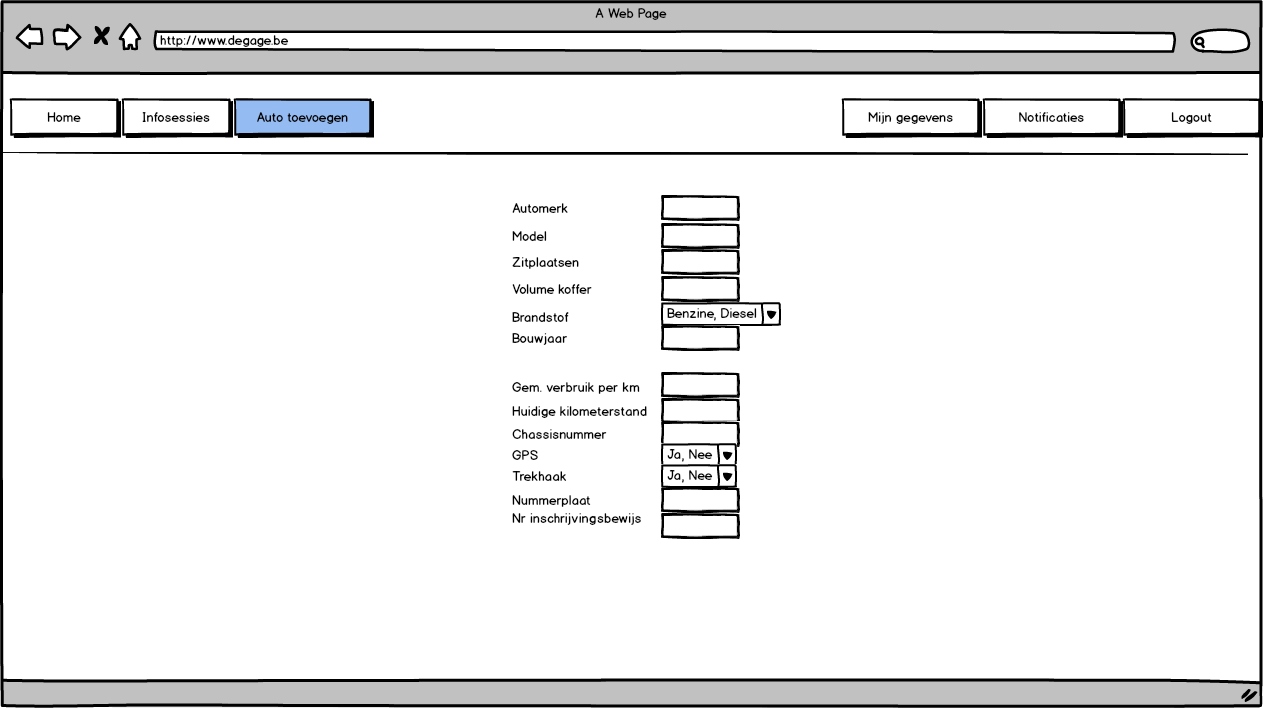
\includegraphics[width=\textwidth]{../../mockups/registratie_eigenaar_auto.png}\end{figure}

\subsection{Zone kiezen bij auto lenen}
\begin{figure}[H]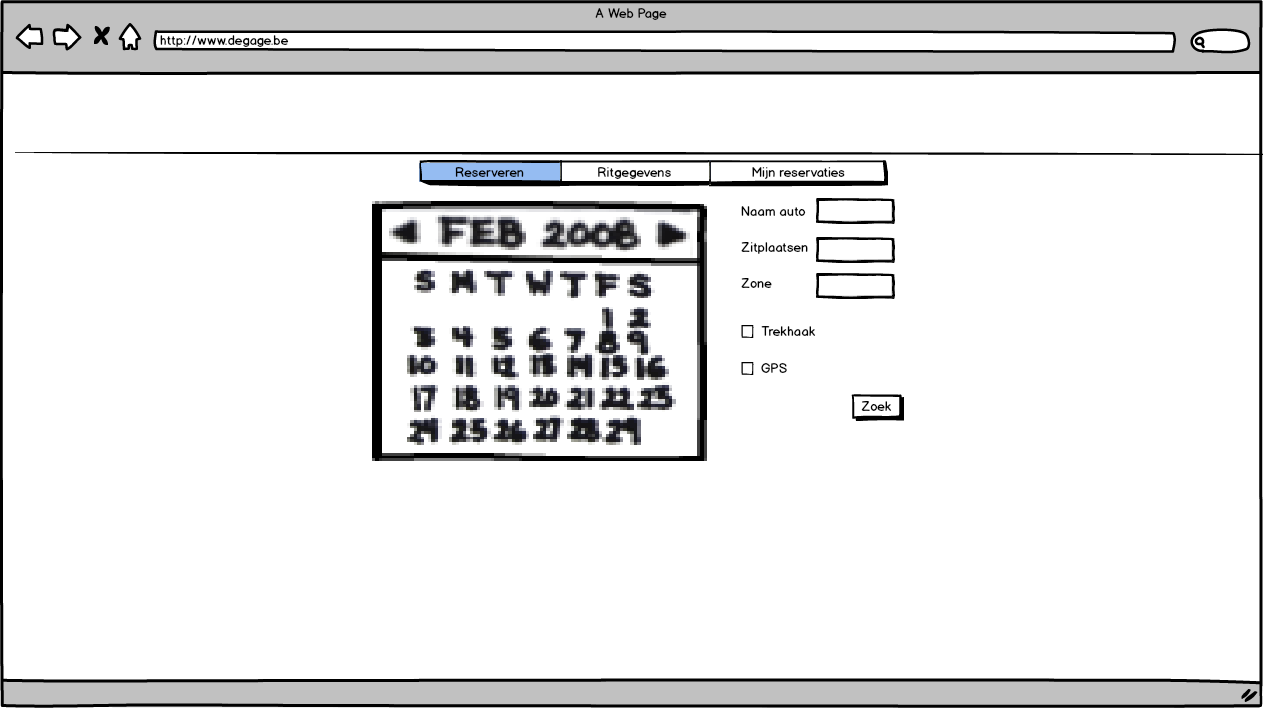
\includegraphics[width=\textwidth]{../../mockups/delen_reserveren.png}\end{figure}

\subsection{Dashboard om vlot te navigeren naar de belangrijkste functionaliteiten voor iedere soort gebruiker}
\begin{figure}[H]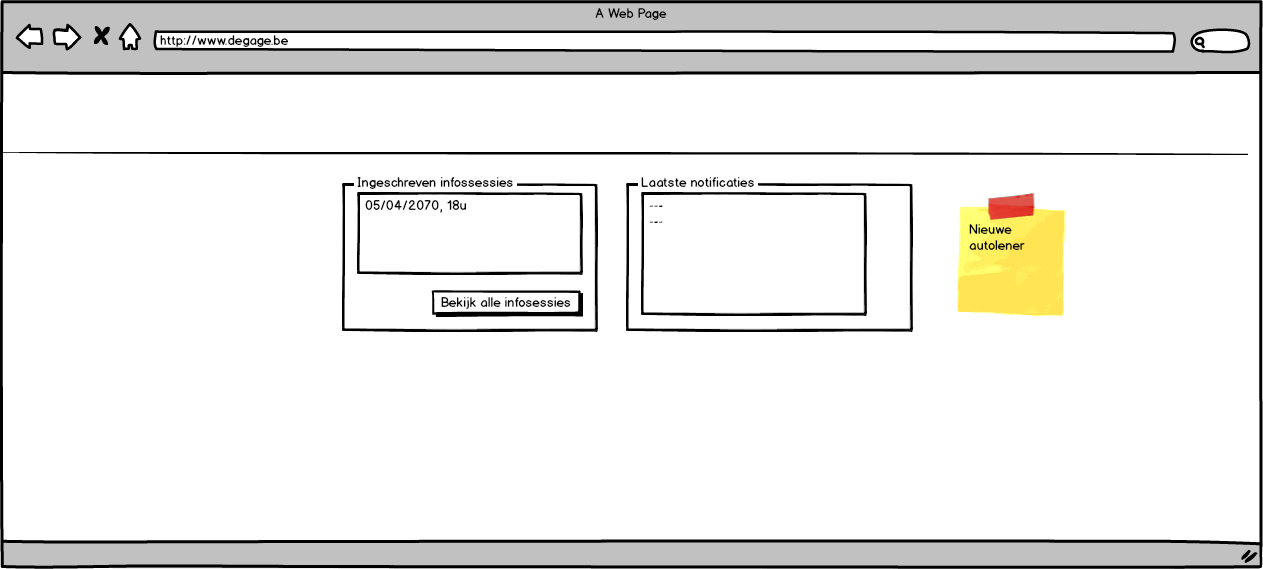
\includegraphics[width=\textwidth]{../../mockups/dashboard_newcaruser.png}\end{figure}
\begin{figure}[H]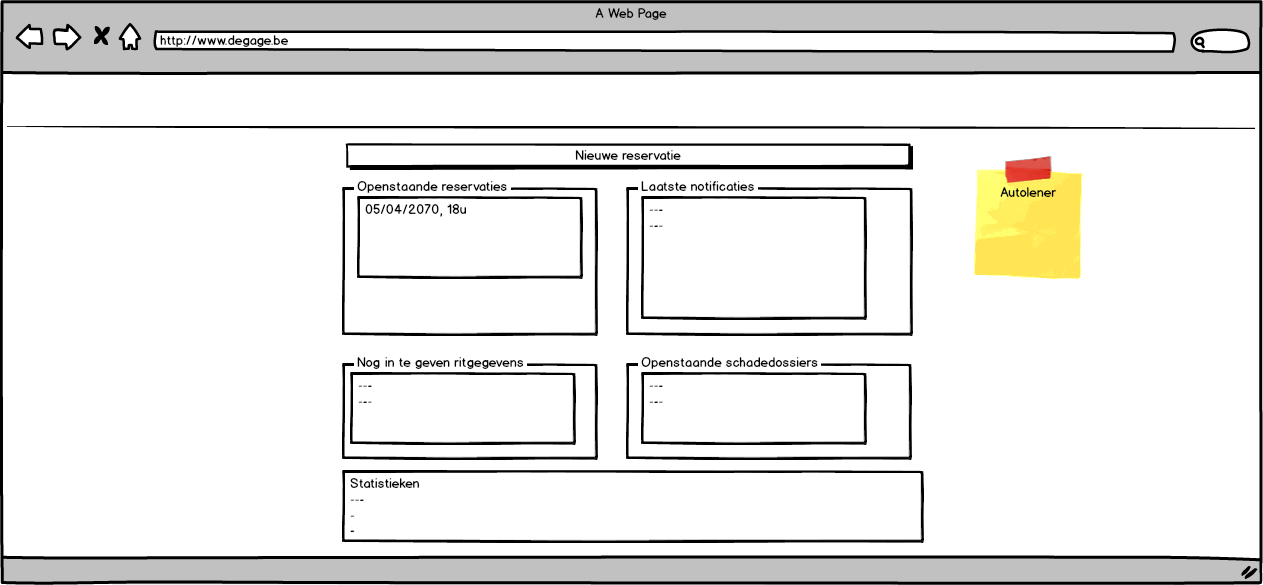
\includegraphics[width=\textwidth]{../../mockups/dashboard_caruser.png}\end{figure}
\begin{figure}[H]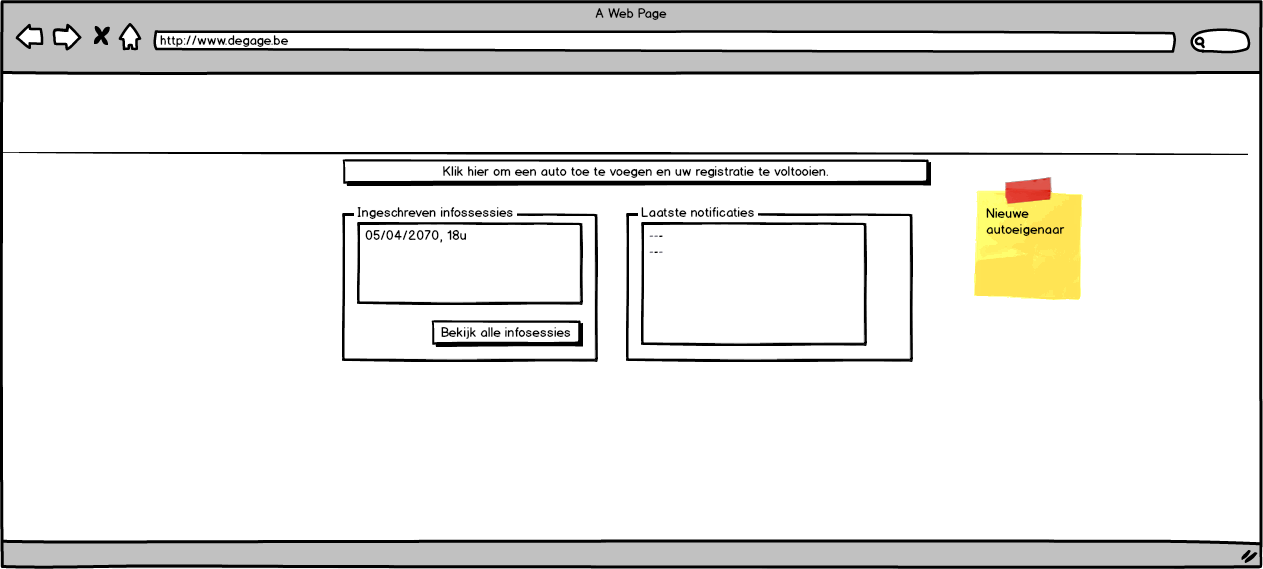
\includegraphics[width=\textwidth]{../../mockups/dashboard_newcarowner.png}\end{figure}
\begin{figure}[H]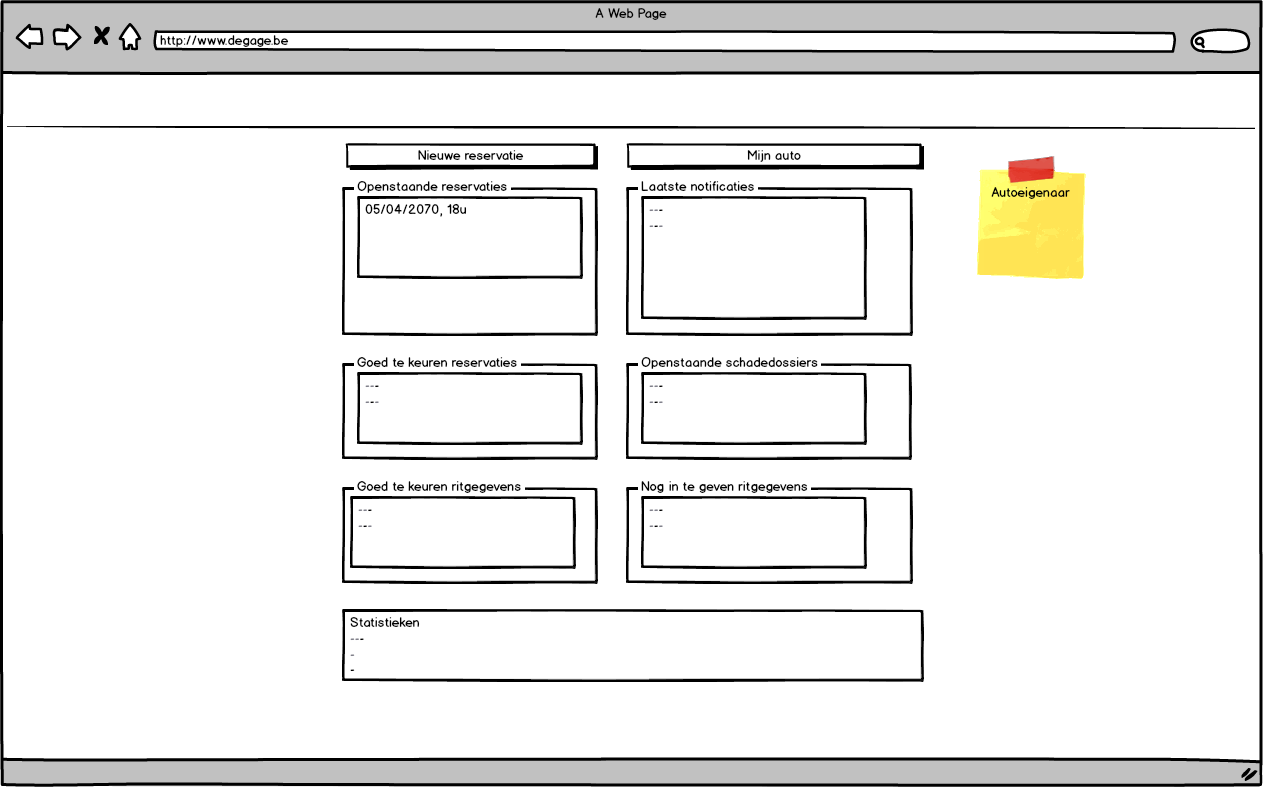
\includegraphics[width=\textwidth]{../../mockups/dashboard_carowner.png}\end{figure}
\begin{figure}[H]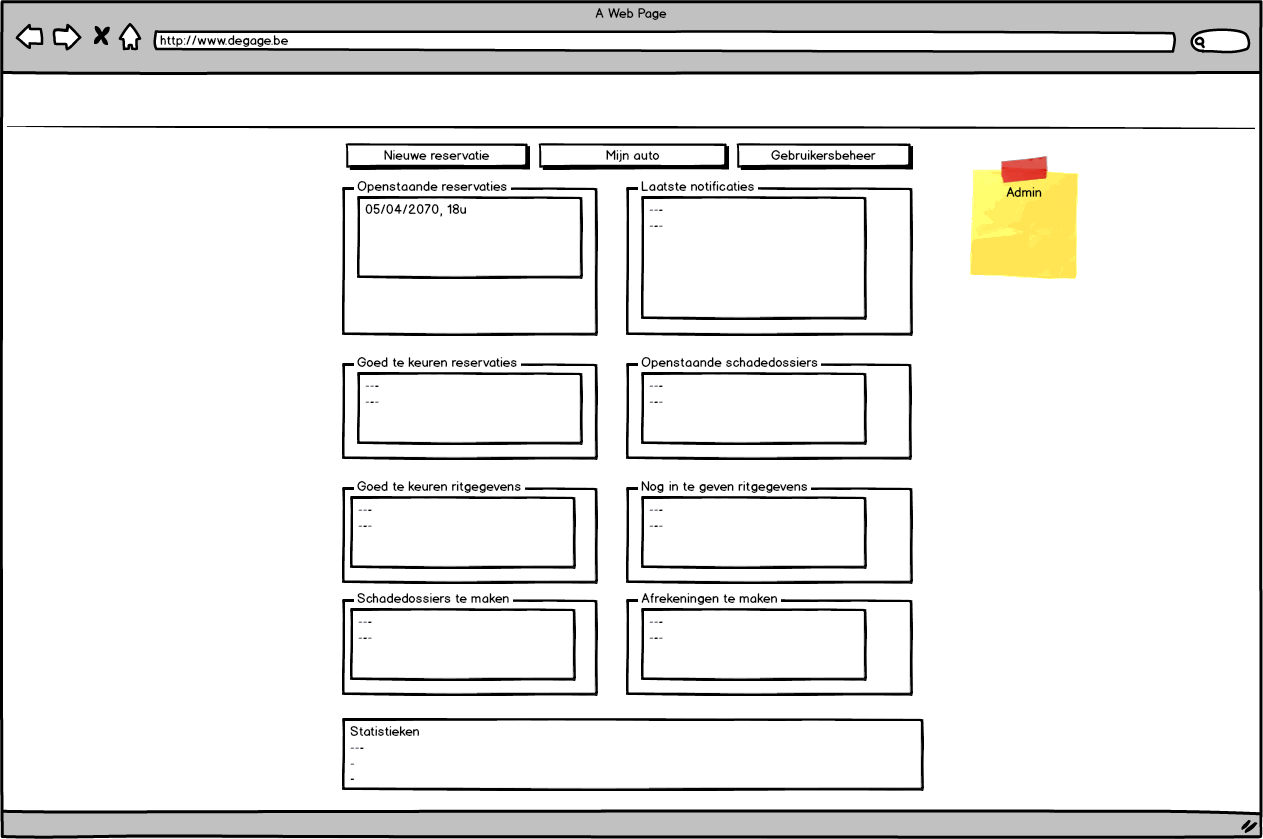
\includegraphics[width=\textwidth]{../../mockups/dashboard_admin.png}\end{figure}

\subsection{Duidelijkere keuzes voor de admin}
\begin{figure}[H]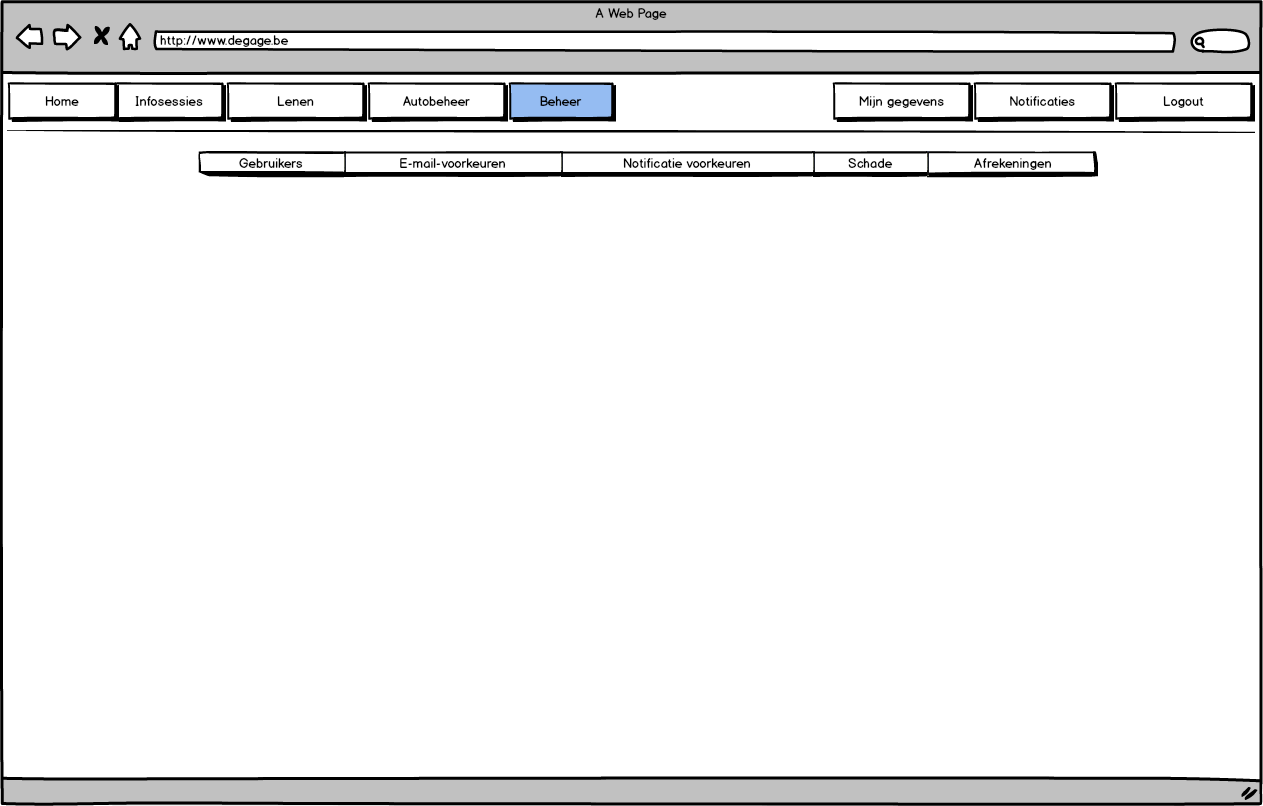
\includegraphics[width=\textwidth]{../../mockups/admin_menu.png}\end{figure}

\subsection{Schadedossiers doorzoeken per gebruiker en per auto}
\begin{figure}[H]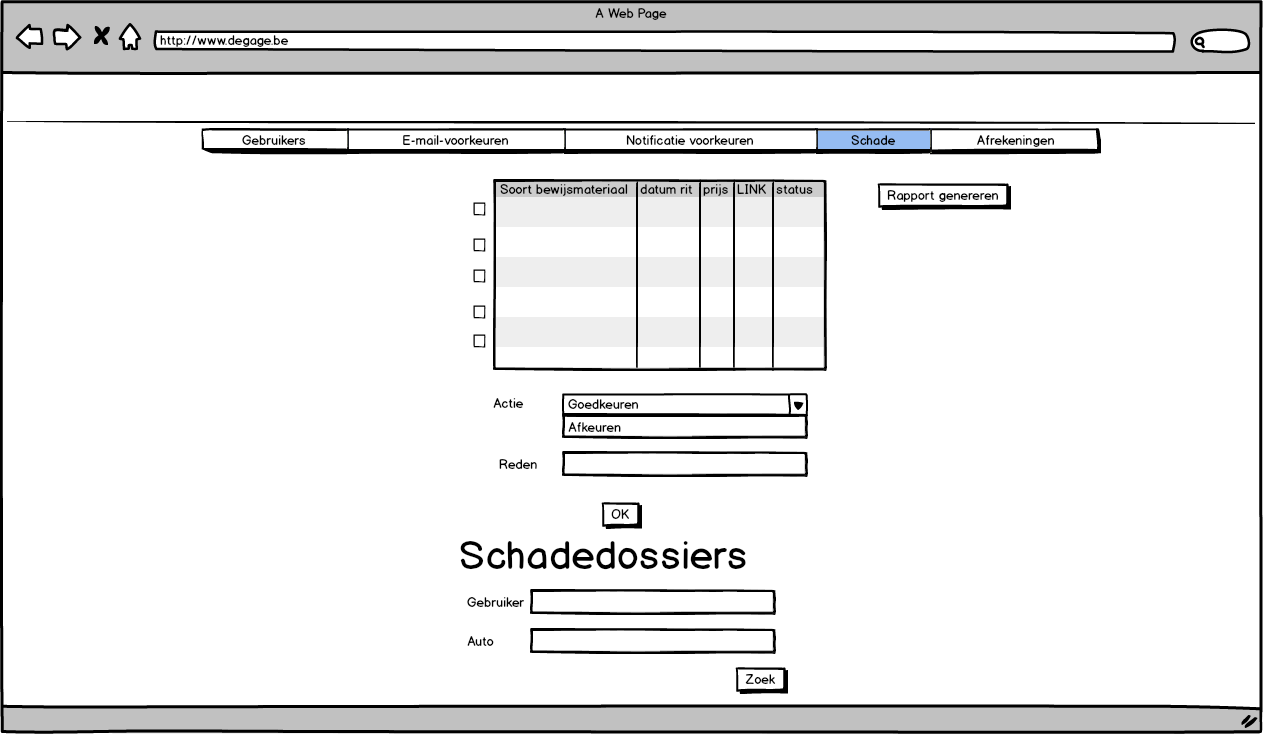
\includegraphics[width=\textwidth]{../../mockups/admin_schade.png}\end{figure}

\subsection{Details van een gebruiker bekijken}
\begin{figure}[H]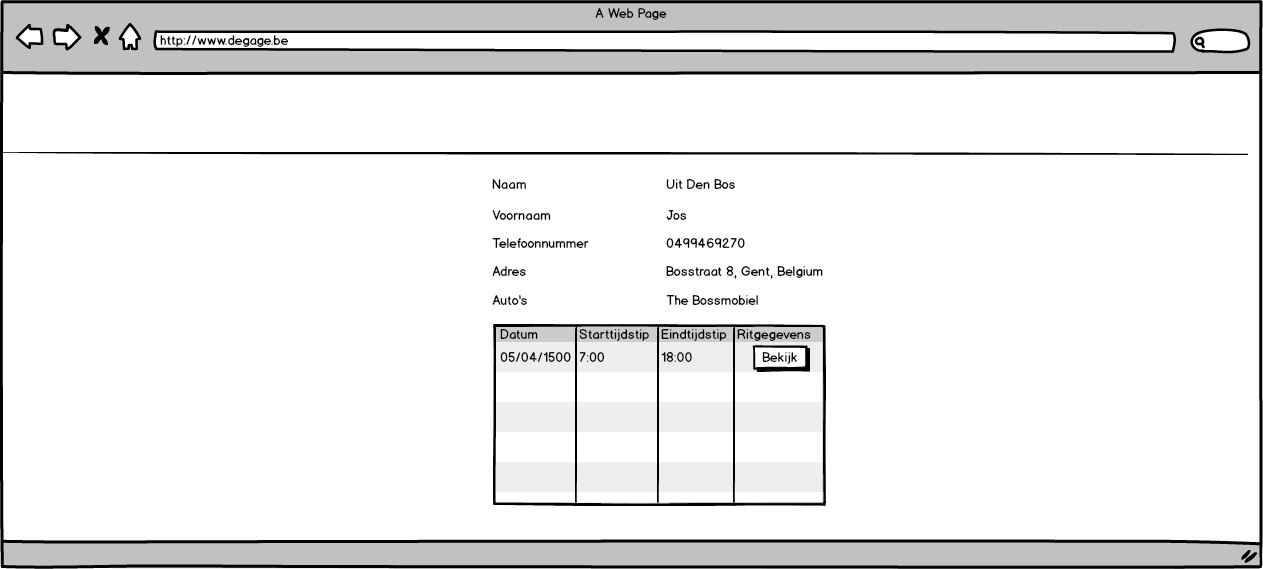
\includegraphics[width=\textwidth]{../../mockups/gebruiker_profiel.png}\end{figure}




\end{document}
